\documentclass[12pt,a4paper]{article}
\usepackage{times}
\usepackage[english]{babel}
\usepackage{durhampaper}
\usepackage{harvard}
\usepackage{graphicx}
\usepackage{fontspec}

\newfontface\lserif{Liberation Serif}

\newcommand{\Csh}{C{\lserif\#}}

\newcommand{\deliverable}[2]{\item \textbf{#1} --- #2}
\newcommand{\layer}[2]{\item \textbf{#1} --- #2\vspace{-1mm}}

\citationmode{abbr}
\bibliographystyle{agsm}

\title{AI for Autonomous Agents in Games and Simulations}
\author{James King}
\student{James King}
\supervisor{Magnus Bordewich}
\degree{BSc Computer Science}

\date{\today}

\begin{document}

\maketitle

\begin{abstract}
These instructions give you guidelines for preparing the final paper.  DO NOT change any settings, such as margins and font sizes.  Just use this as a template and modify the contents into your final paper.  Do not cite references in the abstract.

The abstract must be a Structured Abstract with the headings {\bf Context/Background}, {\bf Aims}, {\bf Method}, {\bf Results}, and {\bf Conclusions}.  This section should not be longer than half of a page, and having no more than one or two sentences under each heading is advised.
\end{abstract}

\begin{keywords}
AI, BDI, cooperative, multi-agent, subsumption, task planning, video game
\end{keywords}

\section{Introduction}
\subsection{Context}\noindent
Video game worlds are often populated with computer controlled Non-Player Characters (or NPCS), the behaviour of which can make or break a game. A great deal of effort is required when designing the routines used by these characters if they are to satisfy the following major requirements. They should behave with approximate rationality, provide an appropriate challenge for the player and act in a believable way if the characters represent humans (or at least animals). For Real-Time Strategy (or RTS) games the difficulty is further accentuated by the necessity for the game to support perhaps hundreds or even thousands of these characters in an environment simultaneously. This combines the previous three requirements with a fourth: performance. Designing solutions for the first three key requirements is often more of a creative task than a purely methodical one and entails an element of subjectivity. The fourth requirement is easier to test, but the difficulty in maintaining a minimum performance quality heavily depends on the complexity of the solutions for the first three goals.

\subsection{Problem Domain}\noindent
This project aims to explore possible implementations of an NPC behaviour system designed to realise the central gameplay of a work-in-progress RTS game. The components of the game that existed prior to this project form a zombie epidemic simulation within a procedurally generated city environment containing buildings separated by streets constructed on a tile-based grid. Initially, a number of human characters are dispersed around the environment, a fraction of which are allocated the role of being a zombie. The simulation then begins, with the zombies navigating towards the nearest visible human and humans attempting to run away from danger if any is present (and otherwise just wandering randomly). If a zombie catches up to a human it may attack it, reducing a stored health value for that human and infecting that human with some probability. A human will become a zombie if they are infected when their health value reaches zero, while a zombie or non-infected human is simply removed from the simulation upon losing all their health.

The conflict is clearly one-sided, not least because the zombies are smarter than the humans. The humans have little regard for their surroundings other than the locations of visible enemies and so often run directly into the inner corners of walls. This would obviously not be classed as a sufficient behaviour as it does not meet the core requirements for a decent NPC. It fails at being rational, at providing an appropriate challenge (the humans don't stand a chance) and the agents certainly don't act like humans. Their only redeeming quality is that their simple AI isn't too computationally expensive, so thousands of them can be supported simultaneously.

\subsection{Project Aims}\noindent
At the very least the artificial intelligence routines explored in this project should improve each human agent's survival ability. This may mean attempting to escape when cornered, deciding when it is rational to attack in self defence and implementing strategies to hide from danger. Later on in the project a player will be able to assign actions for the humans to complete, such as instructing a group to navigate to a specific location, or to construct barricades out of material found in buildings. These commands may conflict with an agent's necessity for self preservation, so the processes developed should intelligently decide when it is rational to neglect an order in favour of reacting to danger.

On the topic of player-specified tasks, an efficient path finding technique will need to be implemented that balances computation time with optimality of the path found. This algorithm will be essential for when agents are directed to a specified location by the player, but also useful for attempting to navigate when performing other tasks or to detect if a path exists to bypass some barricades (thereby establishing whether they are secure). Some tasks may not be assigned to a specific agent but will rather be goals to be achieved by the collective group. For example, the player will be able to instruct that a barricade should be built in a specific location. In this instance the human agents should automatically distribute sub-tasks between themselves in order to achieve the common goal efficiently.

The two core approaches to be compared are a Subsumption architecture \cite{brooks90} and a Belief-Desires-Intentions model \cite{rao95}. A subsumption architecture features a stack of behaviour layers where each may in turn choose to either act or subsume control to the next layer, starting with the top of the stack. The first layer in the sequence to specify an action is heeded and the rest are ignored. This design usually relies on complex behaviour emerging from complimentary layers. A Belief-Desires-Intentions model is a radically different approach, where each agent records an internal representation of the world from which a set of attainable goals are found, a subset of which are committed to in an attempt to maximise expected utility.

\subsection{Deliverables}\noindent
These following core elements will be created before the end of the project.

\begin{enumerate}
  \deliverable{Expanded Core Game}
  {The main environmental components that the AI system will interact with must be implemented. These include the creation of game objects that represent a resource to be used when building barricades, the system to support the construction of the barricades themselves and an expanded user interface which allows a player to select groups of agents and assign tasks. Additionally facilities to be used by the two proposed architectures should be provided, such as a path-finding implementation.}

  \deliverable{Subsumption Prototype}
  {An agent design using a subsumption architecture will be developed, implementing the core requirements of the human NPCs. This prototype will be constructed by breaking up the humans functionality into a stack of behaviours, from which a successful strategy is designed to emerge. Relies on deliverable 1.}

  \deliverable{BDI Prototype}
  {A distinct agent design using a BDI architecture will also be developed, meeting the same requirements as the subsumption approach. This prototype will use a personal abstracted representation of the environment for each human agent, from which a set of achievable goals are found using a goal evaluation algorithm. These goals are then further reduced into a set that is calculated to yield the most utility and are simultaneously possible. Relies on deliverable 1.}

  \deliverable{Analysis \& Final Report}
  {Both completed prototypes will be analysed and compared in terms of agent survival rate (without player intervention), efficiency at which goals specified by a player are achieved, prevalence of unnatural behaviour and system resource usage. The results of this comparison will be compiled into a report, along with the identification of the prototype that is most suited for the problem and an explanation for why that prototype was chosen. The report will also cover possible areas of additional research exposed by this project. Relies on deliverables 2 and 3.}
\end{enumerate}

\section{Related Work}
This section presents a survey of existing work on the problems that this project addresses.  it should be between 2 to 4 pages in length.  The rest of this section shows the formats of subsections as well as some general formatting information for tables, figures, references and equations.

\subsection{Main Text}

The font used for the main text should be Times New Roman (Times) and the font size should be 12.  The first line of all paragraphs should be indented by 0.25in, except for the first paragraph of each section, subsection, subsubsection etc. (the paragraph immediately after the header) where no indentation is needed.

\subsection{Figures and Tables}
In general, figures and tables should not appear before they are cited.  Place figure captions below the figures; place table titles above the tables.  If your figure has two parts, for example, include the labels ``(a)'' and ``(b)'' as part of the artwork.  Please verify that figures and tables you mention in the text actually exist.  make sure that all tables and figures are numbered as shown in Table \ref{units} and Figure 1.
%sort out your own preferred means of inserting figures

\begin{table}[htb]
\centering
\caption{UNITS FOR MAGNETIC PROPERTIES}
\vspace*{6pt}
\label{units}
\begin{tabular}{ccc}\hline\hline
Symbol & Quantity & Conversion from Gaussian \\ \hline
\end{tabular}
\end{table}

\subsection{References}

The list of cited references should appear at the end of the report, ordered alphabetically by the surnames of the first authors.  References cited in the main text should use Harvard (author, date) format.  When citing a section in a book, please give the relevant page numbers, as in \cite[p293]{budgen}.  When citing, where there are either one or two authors, use the names, but if there are more than two, give the first one and use ``et al.'' as in  , except where this would be ambiguous, in which case use all author names.

You need to give all authors' names in each reference.  Do not use ``et al.'' unless there are more than five authors.  Papers that have not been published should be cited as ``unpublished'' \cite{euther}.  Papers that have been submitted or accepted for publication should be cited as ``submitted for publication'' as in \cite{futher} .  You can also cite using just the year when the author's name appears in the text, as in ``but according to Futher \citeyear{futher}, we \dots''.  Where an authors has more than one publication in a year, add `a', `b' etc. after the year.

\section{Solution}

\subsubsection{Development Environment}\noindent
The original game that this project is extending is written in \Csh, so that will be the primary programming language used. Microsoft's Visual Studio 2013 will be used as an integrated development environment for its \Csh~compiler, debugging and profiling tools and Sublime Text 2 for any peripheral text editing. Development will mainly be on a Windows desktop PC (Intel Core i5, AMD 7850), using a Windows laptop (Intel Core i7, nVidia GeForce GT 540M) to test performance on a device with an nVidia GPU. The OpenTK library is used to expose OpenGL bindings for .NET and is the only non-standard library used.

\subsubsection{High Level Architecture}\noindent
Currently, after the environment has been generated a main control loop begins. During each iteration this loop will either perform a simulation step, redraw the screen, or both; depending on how much time has passed since those respective actions were last performed. While screen redrawing will occur as frequently as possible while maintaining a minimum period of 16.67ms, simulation steps attempt to maintain an average period of that same frame-time. This may involve running slightly more simulation steps than the desired average to make up for a prior period of slow updates that fell below the average. Each simulation step cycles through every object in the game environment, including agents, and allows them to perform some individual logic. Following this, player inputs are interpreted and some additional processing will be performed as described in sections \ref{sec:paths} and \ref{sec:bdi}.

\subsubsection{Path Finding \& Navigation}\noindent
The problem of finding efficient paths through virtual environments is often faced when developing AI for games and so has been explored extensively. Generally the A* algorithm \cite{bulitko10} or one of the many variants is used, although while it guarantees a high quality path it may require a significant amount of time to find it (depending on the complexity of the environment). When observing the structure of the worlds produced by the procedural city generation algorithm (See Figure~\ref{fig:block}) it is easy to spot aspects that could potentially be exploited to produce an A* adaptation which required less time to execute.

\label{sec:paths}
\begin{figure}[h]
\centering
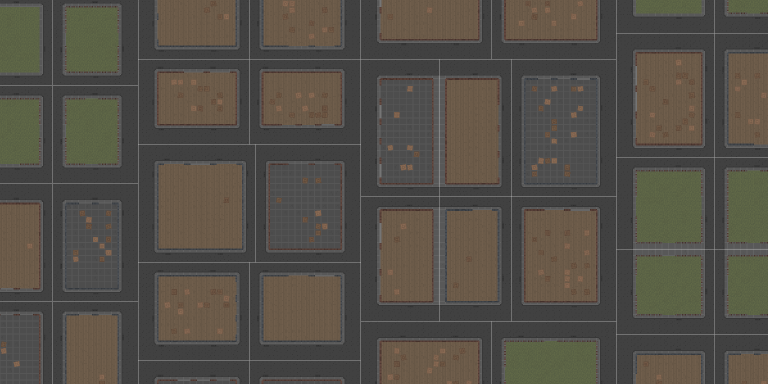
\includegraphics[width=0.9\textwidth]{blocks}
\caption{A diagram to show the structure of a procedurally generated city environment, featuring blocks of buildings separated by roads. Each block is bounded by a white rectangle.}
\label{fig:block}
\end{figure}

When imagining how we would solve the problem of navigating to a remote position in a city in the real world, we don't think on a metre-by-metre basis. We plan our overall route street-by-street and only worry about how to navigate down each road when we reach it. A similar approach can be implemented here, where an agent first applies the A* algorithm on a graph representing the road network of the city and then applies a more refined A* instance along each street when it reaches it as described by \citename{buro05} \citeyear{buro05}. A refined path is also found from the agent's initial position to the nearest street and then from the final street to the destination. For cases where the street-based route takes a corner, the refined A* instance should look for paths between the start of the street preceding corner to the end of the street following it, in case the block that they share a border with can be cut across.

One of the requirements of the system was for it to maintain a minimal amount of processing time per simulation step. This may still be exceeded if many agents calculate refined paths during the same step, so a queueing system should be implemented to limit the number of paths determined per iteration. Each agent that wishes to find a refined path will submit a request to the back of a shared queue while removing any of their previous requests. Once per simulation step this queue will be processed, dequeuing and servicing requests until some time limit is exceeded. This process should occur after all individual agent calculations are complete, so that this time limit can accommodate those agent actions. This may mean that several simulation steps will be required for a large group of agents to receive paths, but distributing this processing time over several frames is obviously preferable to the game pausing for a visible amount of time. As an additional positive side effect, seeing a crowd of instructed agents begin to move at different times over a few frames would appear more natural than them all moving simultaneously.

This algorithm should produce results very close in length as to when applying a single instance of refined A* across the entire route, with a far shorter execution time for all but the most trivial instances. If the implementation still leads to a performance bottleneck then it could potentially be improved by caching the paths found along individual streets, which can then be looked up instead of calculating the same paths multiple times. This will be particularly beneficial when a large group of nearby agents are travelling to the same destination.

\subsubsection{Vision \& Collision Testing}\noindent
Visibility testing and collision detection are similar problems and can be largely solved with the same algorithm. For collision detection the program is testing if an object (simplified as its bounding rectangle)
can be `swept' along a vector representing the movement it wishes to make during the current simulation step. If the swept rectangle intersects with solid world geometry, the object's movement is pulled back to the furthest it could go without such an intersection. Similarly, when testing the visibility of an object you are essentially testing whether it can be swept towards the observer without being blocked by any solid geometry, thereby detecting if its image would be blocked by a wall.

This sweeping action is the costly part of the technique, an optimal solution will limit the number of intersections tested with this swept area to the absolute smallest number required. As in this scenario only walls can intersect the object, and walls are only present along the edges of tile, the distance along the movement vector that the object is swept can be incremented by amounts that exactly move it to the next tile boundary that would be met. This method is illustrated by Figure~\ref{fig:trace} and is an adaptation of the technique used in early 3D environment rendering \cite{raycast}.

\begin{figure}[h]
\centering
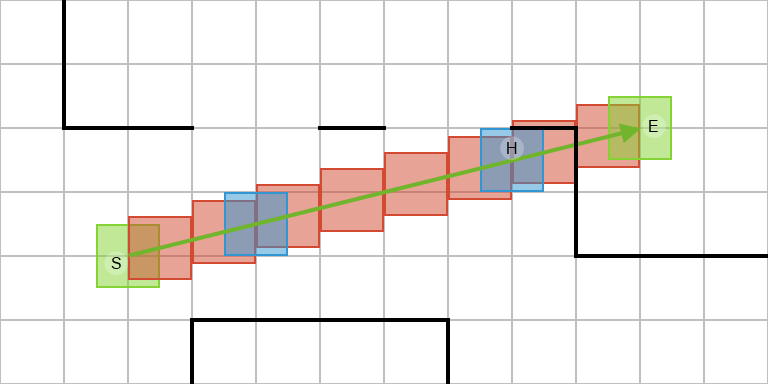
\includegraphics[width=0.9\textwidth]{trace}
\caption{A diagram to show the world geometry intersection checks performed when sweeping an object's bounding rectangle along a trace line. The object starts at position $S$ and its destination is position $E$. Black lines represent solid walls. The red boxes show iteration steps where a horizontal collision test is performed against possible obstructions to the right and the blue boxes are iteration steps where vertical collision tests are performed upwards. Position $H$ is the projected box location where a collision is first detected and so will be the position the object is moved to.}
\label{fig:trace}
\end{figure}

This technique compares well against the usual na\"{i}ve approach of sweeping a certain fixed distance along the movement vector each iteration. It is guaranteed to find an intersection if one exists and calculate the exact distance the object would have to travel to reach it rather than just the previous iteration location when using a constant step distance. It also requires fewer iterations, assuming a constant step distance approach uses a small iteration delta (which it would need to for accurate results).

\subsubsection{Subsumption Prototype}\noindent
Central to a subsumption agent architecture is a stack structure upon which behaviour layers can be pushed. This is relatively simple to implement using an Object Oriented approach and an adaptation of the design used by \citename{butler01} \citeyear{butler01} will be used involving an abstracted behavioural layer class with a method to be overridden called when that layer should decide to act. This method will return $true$ if an action is performed by that layer, otherwise $false$. The highest layer in the stack will be invoked first and if that layer returned $false$ the next layer will be invoked. This continues until either a layer returns $true$, or the last layer has been invoked. The proposed layers to be implemented are listed below, with the top-most layer first.

\noindent
\small{
\begin{itemize}
\layer{DropResource}{Drop a carried resource if in danger or at a barricade under construction}
\layer{SelfDefence}{Attack a pursuer if they are too close}
\layer{Mob}{If there are many more humans than zombies nearby, head towards a zombie}
\layer{VacateBlock}{If carrying a resource or in danger while inside a building, run outside}
\layer{Flee}{Run away from nearby danger}
\layer{FollowRoute}{Follow a route assigned to this agent}
\layer{PickupResource}{If standing on a resource and not in danger, pick it up}
\layer{FindResource}{If not in danger and not holding anything, move towards a resource}
\layer{HarvestResource}{Attack a nearby object that yields resources when broken}
\layer{SeekRefuge}{When outside and neighbouring a safe-looking building, run inside it}
\layer{Wander}{Walk around randomly}
\end{itemize}}

This particular configuration of behaviours should satisfy each requirement of the AI prototype, using complimentary sets of layers to allow for more complex compound behaviours to emerge. The survival strategy is implemented with the $SelfDefence$, $Mob$, $VacateBlock$, $Flee$ and $SeekRefuge$ layers, $FollowRoute$ for travelling to player designated locations and the remainder (along with $VacateBlock$ and $SeekRefuge$ again) for constructing barricades autonomously.

The survival aspect functions with several emergent sub-strategies. The $SelfDefence$ behaviour will attack a zombie that is extremely close to the agent, which is expected to occur when the zombie catches up to the agent due to a movement speed advantage or if the agent has been chased into a corner. In either case, attacking the pursuer is the only rational thing left to do. The $Mob$ behaviour actively directs an agent towards a nearby zombie if that agent predicts that a decent number of other agents will perform the same action, enough to overwhelm the zombie. When the agents are close enough, the $SelfDefence$ behaviour will take control and cause the agents to attack the surrounded enemy. This strategy should lead to zombies being eliminated in safe situations where it is unlikely for a human agent to take much damage. $VacateBlock$ and $Flee$ will help avoid situations where being in close proximity to a zombie is unnecessary and $SeekRefuge$ ensures agents aren't exposed outside.

Barricade construction relies on a similar interaction between several behaviours. The process usually starts with an agent wandering around outside, carrying no resource object. The $SeekRefuge$ behaviour will lead it to navigate inside a building, within which it may find objects that yield resource items when damaged when obeying the $HarvestResource$ behaviour. When the object breaks into its component resources, the $PickupResource$ behaviour is followed and the agent now holds a resource item. The $VacateBlock$ layer instructs the agent to leave the building if it is holding a resource and as soon as the agent leaves it drops the item as instructed by the $DropResource$ layer. The agent then attempts to $SeekRefuge$ again and the cycle repeats. Resource items are continually dropped onto tiles neighbouring an exit to the building, which pile up to form barricades. When the barricade becomes large enough, the tile it belongs to becomes solid and the agent automatically finds a different path to leave and re-enter the building, thereby dropping items onto a different tile.

This solution is quite trivial to implement due to the simplicity of each individual layer. Some behaviours, such as $Mob$ and $Flee$, provide some scope for experimentation by testing different thresholds for when to perform that action. Additionally, it may be interesting to test whether agents survive longer if they all posses the $Mob$ layer, or if having a subset of agents that deviate from that strategy will lead to that set lasting markedly longer than the longest surviving agents in the first instance.

\subsubsection{BDI Prototype}\noindent
For a BDI agent architecture we must design each of the three core components (Beliefs model, Desires identification and Intentions filtering) as individual systems \cite{rao95}. After this, for each type of intention a planning mechanism must be implemented.

The Beliefs component involves designing a system for representing aspects of an agent's environment that could influence its actions, updating that internal representation as the agent perceives stimuli. The most direct structure for this model of the environment (while guaranteeing that potentially useful information is stored) would be to store every detail exactly as it is perceived; but this would be difficult to parse, would hold unnecessary detail and could result in too much memory being consumed. A better approach would be an abstracted model, perhaps considering two levels of abstraction as with the path-finding solution (see section~\ref{sec:paths}). The highest level abstraction will be at a city block scale, considering observed attributes of the contents of each block. Each agent will track a few key properties about each block; the last time they observed it, whether that block contains a building, the number of human agents seen within that block, the number of zombie agents and the number of barricade resources seen. Each agent will also track the locations of observed agents and resources for their local environment, information that will be discarded when they travel a specified distance from those locations to save memory. Agents will also record whether they are within a building or outside, their health value and whether they are holding an item.

Desire identification is the next component requiring planning, which involves designing a mechanism to parse the beliefs model to find a set of achievable goals that align with the higher aspirations of the agent. For this specific scenario, these aspirations will be to improve safety and achieve player-given tasks. These high level goals can be broken down into sub-goals as described by Figure~\ref{fig:goals}.

\label{sec:bdi}
\begin{figure}[h]
\centering
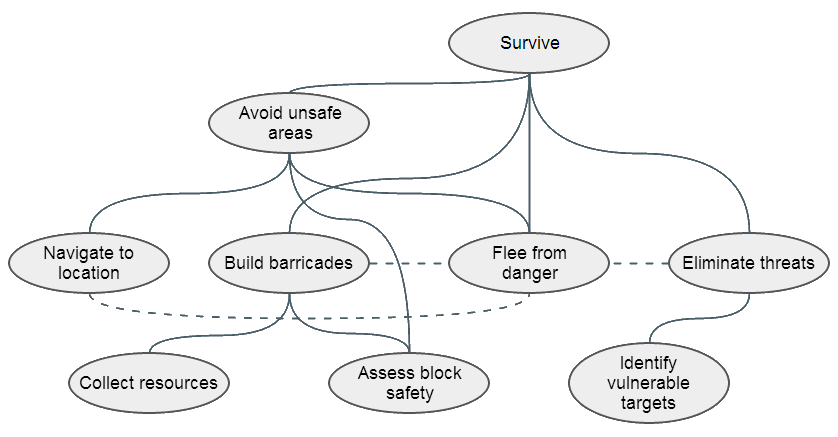
\includegraphics[width=0.8\textwidth]{goals}
\caption{A diagram to show a breakdown of the main goals for a human agent into sub-goals, with possible conflicts signified by dashed lines.}
\label{fig:goals}
\end{figure}

The \emph{Avoid unsafe areas} sub-goal obviously relies on being able to identify whether an area is potentially hazardous and more importantly whether there is another location worth travelling to due to increased expected safety. Implementing this can exploit the abstracted block-level representation of the world as defined in the Beliefs model by calculating a \emph{danger} heuristic for each block. This heuristic would be a function of the remembered number of zombies, humans, barricade resources and taking into account uncertainty related to the amount of time since the block was last observed. The details for specifically how these values are manipulated into forming the heuristic will be a point for experimentation, as it will be difficult to discover the optimal way to factor in uncertainty without testing. A second heuristic should then be calculated for each block which finds the estimated cost of travelling there, determined with an A* instance that uses the values from the previous heuristic as edge weights for path segments travelling through each block. If any blocks are deemed to be safer than the one the agent currently resides in (using the first heuristic) and is also found to be worth the trip (using the second heuristic), the agent will desire to travel to it.

For the \emph{Eliminate threats} sub-goal, agents need to rely on teamwork to safely and efficiently attack zombies. A one-on-one fight will lead to the human receiving a considerable amount of damage, whereas if a large group of humans attack an individual target the fight will be resolved quickly before much damage is dealt by the zombie. For this cooperative strategy to work, agents need to determine if enough other agents will be willing to pitch in for the battle to be worth undertaking. This can be achieved by each agent independently being empathetic towards other agents within a certain range of the prospective target, asking ``if I was that agent, would I attack the target assuming all other nearby agents attacked too?'' If it is estimated that a sufficient number would cooperate, a desire to attack the target would be included with the desire set. As a fail-safe for when guessing the intentions of other agents fails, if an agent finds itself considerably closer to a zombie than other agents it will forfeit the desire to attack it in favour of desiring to flee.

Forming desires related to the construction of barricades relies on there being a known local position requiring one, either through finding a constricted space that would require a small barricade to produce a large enclosed area, or identifying a location that has been requested by a player to have a barricade. The former situation has a trivial solution in that the entrances to buildings are easy to recognise for an agent, but an ideal solution would also eventually construct barricades across streets to enclose several safe city blocks as a human stronghold. This can be implemented through incrementally expanding existing enclosures; initially a building will be be barricaded across its entrance, then barricades are constructed across the ends of the street that the entrance looks upon (with the original barricade then being de-constructed) and then the barricade extends outwards to claim more streets that were previously exposed (see Figure~\ref{fig:barricades}). When the location for a barricade has been identified by an agent, it will desire to construct it. The barricades will be left on the cusp of completion, allowing for agents to travel through it, until a threat is detected near to the compromised section.

\begin{figure}[h]
\centering
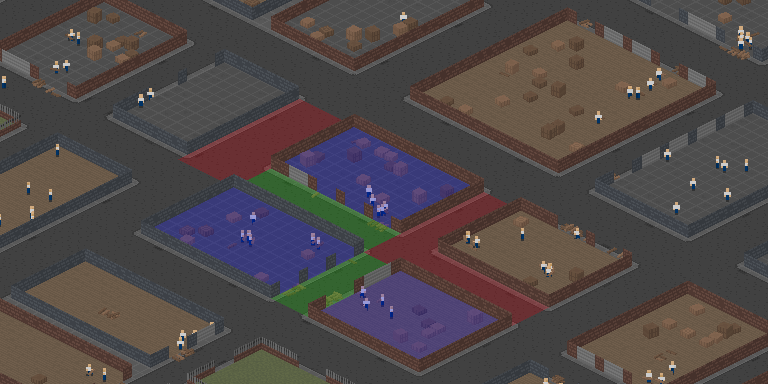
\includegraphics[width=0.9\textwidth]{barricades}
\caption{A diagram to show the proposed automated barricade expansion process. Barricades enclosing single buildings (blue) will initially be produced, followed by an expansion of the enclosure onto the neighbouring street (green) and then progressively outwards to adjacent streets (red). The process will continue in this manner while resources are available and the encroached area houses no threats.}
\label{fig:barricades}
\end{figure}

The intention filtering process attempts to reduce the set of desires into a subset that maximises utility while leaving no conflicting goals (such as desiring to attack a target while also desiring to run away), from which agent actions are then derived. Filtering should prioritise agent survival over task completion and also prefer to travel to a location expected to yield more utility over remaining to build a barricade. Desires to avoid individual threats can be aggregated into a single desire to avoid many threats simultaneously; for example by desiring to leave a building within which are multiple hazards, or treating each enemy as a point charge repelling the agent and desiring to move in the direction of the resulting force vector. This process is expected to be the most performance intensive component of the BDI architecture, so a request queuing system like the one used for refined path calculation should be implemented. Intentions are mostly committed to by an agent for several frames at a time \cite{bonura09}, meaning determining them every simulation step for every agent will be extremely wasteful. Instead, a calculation to determine whether an intention is likely to have changed is expected to be faster to execute and would trigger a request being sent to a shared intention recalculation queue. This queue would be processed once per frame (as will the path calculation process) after all agents have acted, and would dequeue and perform the requested intention determinations until a time limit is exceeded. Obviously it would be more rational for every agent if they could recalculate their intentions immediately after they are believed to have changed, but the simulation step time limit is imperative. Helpfully the appearance of agents within a group ``changing their minds'' at different times from the same stimuli would give a more natural appearance to their behaviour, rather than them all reacting in the same instant.

\subsubsection{Analysis Strategy}\noindent
A comprehensive and fair analytical method is required for comparing the two agent architectures and this section will cover a set of experiments that satisfy both of these qualities.

\textbf{Survival Rate} will be tested by first selecting a set of initial simulation states (at least 10) and running the simulation using each once per agent architecture. Each simulation will be left to run for 5 minutes and the number of survivors and zombies at each moment in time will be logged. The data produced will be used to produce graphs of the agent counts over time which can be analysed in terms of population decline rates, time until a stable population is established and whichever other statistical features that may appear. This test will involve no player interaction, only the purely autonomous aspects of the agent designs.

\textbf{Task Completion} will analyse the efficiency at which each agent design can complete tasks assigned by a player. Similarly to the survival rate test, a set of initial states will be produced over which both architectures will run, the difference being that each initial state will include an instruction to build a collection of barricades at specific locations. The simulation will execute until each barricade is completed, the progress towards completion being recorded over time. This data will be graphed and compared, as with the survival rate data.

\textbf{Performance} of the two architectures is of obvious importance; a solution with optimal survival rate and task completion efficiency has little use if it can only support a handful of agents at a time without reducing the simulation to an agonisingly slow crawl. The main method for the survival rate test can be used here, but with frame-time (the time taken to calculate each simulation step) being recorded rather than survival rate. The main requirement for the architectures is to keep average frame-time below 16.67ms, with minimal dips above that threshold. This test is platform dependant and so will be carried out on at least two different machines. Additional more superficial tests will also be performed with world sizes spanning from 64x64 tiles to 256x256 tiles and a range of agent counts from 50 to 1000 with each world size, to analyse performance relating to dense vs sparse populations.

\section{Results}
\subsection{Quantitative Result Set Acquisition}
Quantitative results were produced by running the subsumptive architecture and two versions of the BDI implementation (one with frequent belief and deliberation updates, and the other with one quarter of the frequency) on a total of 160 different initial world states. These were divided into 8 different categories of world size and initial agent populations, designed to test different population densities, total agent counts, and ratios of survivor agents to antagonistic ones. For each of these categories 20 seeds were used to control the specific geometry generated and placement of agents, giving the total of 160 distinct environments. Figure \ref{fig:environs} lists each of the categories used to produce the final set of results.

\begin{figure}[ht]
\centering
\begin{tabular}{|c|rcl|c|c|} \hline
{\bf Size} & {\bf Survivors} & : & {\bf Zombies} & Agent Ratio & Agent Density \\ \hline
64 & 48 & : & 16 & 3 : 1 & 1.172 \\
64 & 96 & : & 32 & 3 : 1 & 2.344 \\
64 & 120 & : & 8 & 15 : 1 & 2.930 \\ \hline
128 & 96 & : & 32 & 3 : 1 & 0.586 \\
128 & 120 & : & 8 & 15 : 1 & 0.732 \\
128 & 128 & : & 128 & 1 : 1 & 0.781 \\
128 & 192 & : & 64 & 3 : 1 & 1.172 \\
128 & 224 & : & 32 & 7 : 1 & 1.367 \\ \hline
\end{tabular}
\caption{The 8 different initial environment categories, for each of which 20 distinct instances were used for testing. Agent density measures the mean number of survivor agents per 100 tiles.}
\label{fig:environs}
\end{figure}

Each of the 480 individual tests ran for 36,000 individual simulation ticks, which is equivalent to 10 minutes of simulation time at 60 ticks per second. Every time the agent population changed a datapoint would be logged; recording the current time, the number of agents of both types, and the average time spent per tick to simulate the agent AI. The data for each of the 20 instances in a category was then aggregated into a single graph of averaged data, with plots for each AI implementation for comparison.

\subsection{Quantitative Results}
\begin{figure}[ht]
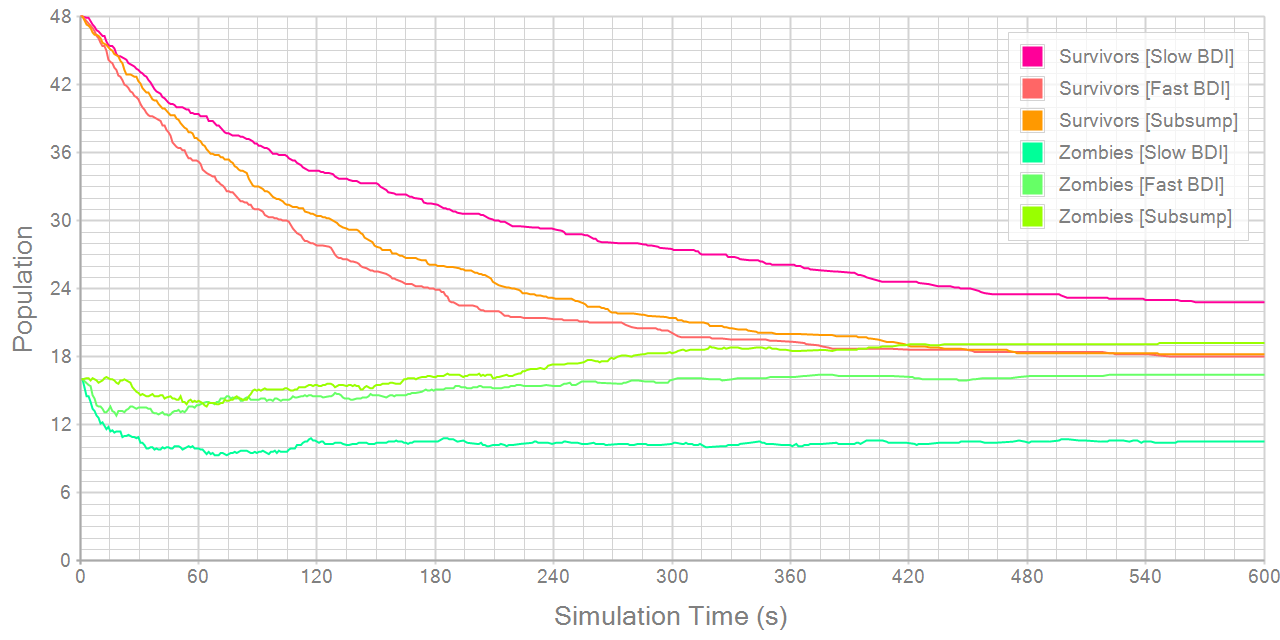
\includegraphics[width=0.9\textwidth]{../../Results/64_48_16/population}
\end{figure}

\section{Evaluation}

This section should between 1 to 2 pages in length.

\section{Conclusions}

This section summarises the main points of this paper.  Do not replicate the abstract as the conclusion.  A conclusion might elaborate on the importance of the work or suggest applications and extensions.  This section should be no more than 1 page in length.

The page lengths given for each section are indicative and will vary from project to project but should not exceed the upper limit.  A summary is shown in Table \ref{summary}.

\begin{table}[htb]
\centering
\caption{SUMMARY OF PAGE LENGTHS FOR SECTIONS}
\vspace*{6pt}
\label{summary}
\begin{tabular}{|ll|c|} \hline
& \multicolumn{1}{c|}{\bf Section} & {\bf Number of Pages} \\ \hline
I. & Introduction & 2--3 \\ \hline
II. & Related Work & 2--3 \\ \hline
III. & Solution & 4--7 \\ \hline
IV. & Results & 2--3 \\ \hline
V. & Evaluation & 1-2 \\ \hline
VI. & Conclusions & 1 \\ \hline
\end{tabular}
\end{table}


\bibliography{projectpaper}


\end{document}